\documentclass[11pt,a4paper]{article}

\usepackage[utf8]{inputenc}
\usepackage[T1]{fontenc}
\usepackage[spanish,es-nodecimaldot]{babel}
\usepackage[a4paper,margin=2.2cm]{geometry}
\usepackage{amsmath,amssymb}
\usepackage{booktabs}
\usepackage{array}
\usepackage{tabularx}
\usepackage{graphicx}
\usepackage{xcolor}
\usepackage{float}
\usepackage{enumitem}
\usepackage{hyperref}
\usepackage{caption}

\graphicspath{{results/}}
\definecolor{tomatored}{HTML}{A52A2A}
\definecolor{darkblue}{HTML}{1D3557}
\hypersetup{colorlinks=true,linkcolor=darkblue,urlcolor=darkblue,citecolor=darkblue}
\setlength{\parindent}{0pt}
\setlength{\parskip}{5pt}
\renewcommand{\arraystretch}{1.15}
\newcommand{\R}{\text{R}}
\newcommand{\G}{\text{G}}
\newcommand{\B}{\text{B}}
\newcommand{\Hh}{\text{H}}
\newcommand{\Ss}{\text{S}}
\newcommand{\Vv}{\text{V}}
\newcommand{\RG}{\text{RG}}
\newcommand{\RB}{\text{RB}}
\newcommand{\GB}{\text{GB}}
\newcommand{\RGB}{\text{RGB}}
\newcommand{\metric}[1]{\num{#1}}

\title{\textbf{Proyecto 1: Segmentación y clasificación\\del estado de madurez de tomates}}
\author{INFO1185: Inteligencia Artificial}
\date{13 de septiembre de 2026}

\begin{document}
\maketitle

\begin{abstract}
Se implementa un sistema reproducible para segmentar tomates mediante K-Means y
clasificar su estado de madurez mediante un clasificador bayesiano gaussiano. El
experimento usa 62 imágenes del conjunto local, 31 maduras y 31 inmaduras, con
partición por imagen y una semilla fija. Se comparan las siete combinaciones no
vacías de los canales RGB mediante Jaccard, se extraen descriptores RGB/HSV, y se
contrastan tres estrategias: Bayes con selección basada en análisis exploratorio,
Bayes con selección secuencial hacia adelante (SFS) y PCA seguido de Bayes.

La mejor combinación de segmentación en desarrollo fue RB, con Jaccard medio
$0.560$. En el test, el mayor AUC correspondió a Bayes + SFS ($0.929$), aunque las
tres estrategias alcanzaron la misma exactitud ($0.846$). PCA retuvo tres
componentes, que explican el $95.16\%$ de la varianza del entrenamiento.
\end{abstract}

\tableofcontents
\newpage

\section{Problema y objetivo}

El objetivo es construir un flujo que reciba una imagen RGB de uno o más tomates,
separe automáticamente el fruto del fondo y determine si el tomate pertenece a la
clase \emph{maduro} o \emph{inmaduro}. El trabajo combina:

\begin{enumerate}[leftmargin=1.5em]
    \item aprendizaje no supervisado para producir la máscara del fruto mediante
    K-Means;
    \item extracción de características únicamente dentro de la máscara estimada;
    \item selección de variables por dos estrategias distintas;
    \item decisión bayesiana con umbral seleccionado en validación;
    \item reducción de dimensionalidad mediante PCA y comparación final.
\end{enumerate}

El flujo experimental es:

\begin{center}
\fbox{\parbox{0.91\textwidth}{
Imagen RGB/RGBA $\rightarrow$ redimensionamiento común $\rightarrow$ K-Means
para $\R$, $\G$, $\B$, $\RG$, $\RB$, $\GB$ y $\RGB$ $\rightarrow$ Jaccard
contra anotación $\rightarrow$ características RGB/HSV del fruto $\rightarrow$
selección o PCA $\rightarrow$ Bayes $\rightarrow$ umbral de Youden $\rightarrow$
test final.
}}
\end{center}

\section{Datos y protocolo experimental}

\subsection{Estructura observada}

El directorio contiene dos clases, \texttt{ripe} y \texttt{unripe}. Cada clase
contiene un subdirectorio \texttt{images} y otro \texttt{masks}; para cada imagen
se encontró exactamente una máscara con el sufijo \texttt{\_mask.png}. La tabla
resume la inspección de los archivos.

\begin{table}[H]
\centering
\caption{Estructura del conjunto de datos.}
\begin{tabular}{lr}
\toprule
Elemento & Resultado \\
\midrule
Imágenes totales & 62 \\
Tomates maduros / inmaduros & 31 / 31 \\
Máscaras encontradas & 62 de 62 \\
Canales originales & 60 RGB y 2 RGBA \\
Altura original & 200--5200 píxeles \\
Ancho original & 250--7792 píxeles \\
Área anotada media, maduro & 0.399 \\
Área anotada media, inmaduro & 0.315 \\
\bottomrule
\end{tabular}
\end{table}

Las resoluciones son heterogéneas y las imágenes RGBA se convierten a RGB
descartando el canal alfa. Para controlar costo y mantener el experimento
reproducible, cada imagen y su máscara se redimensionan manteniendo la proporción
hasta un lado máximo de 256 píxeles. La máscara usa interpolación del vecino más
cercano; la imagen usa interpolación de área. No se mezclan píxeles de una imagen
con otra.

\subsection{Partición y control de fuga de información}

La partición se hace antes de extraer características y por imagen, no por píxel.
Se emplea la semilla $20260913$ y estratificación por clase. Por redondeo entero,
la partición obtenida es cercana a 60/20/20:

\begin{table}[H]
\centering
\caption{Partición estratificada por imagen.}
\begin{tabular}{lrrr|r}
\toprule
Clase & Entrenamiento & Validación & Test & Total \\
\midrule
Maduro & 18 & 7 & 6 & 31 \\
Inmaduro & 18 & 6 & 7 & 31 \\
\midrule
Total & 36 & 13 & 13 & 62 \\
Porcentaje & 58.1\% & 21.0\% & 21.0\% & 100\% \\
\bottomrule
\end{tabular}
\end{table}

La segmentación, la selección de características y PCA se fijan usando solamente
entrenamiento y/o validación. El umbral se selecciona sobre validación y el modelo
final se reentrena con entrenamiento más validación antes de evaluar una sola vez
el test. El conjunto de test no participa en decisiones de diseño.

\section{Exploración de datos}

La exploración de color usa las máscaras de referencia solo para describir la
diferencia entre fruto y fondo durante desarrollo. Para cada imagen se calculan
estadísticos de los píxeles de la región anotada y del complemento. La tabla muestra
promedios sobre las imágenes de entrenamiento y validación.

\begin{table}[H]
\centering
\scriptsize
\caption{Promedios de píxel en desarrollo. H está en grados y S/V en $[0,1]$.}
\begin{tabular}{llrrrrrr}
\toprule
Clase & Región & R & G & B & H & S & V \\
\midrule
Maduro & Fruto & 189.17 & 71.61 & 42.68 & 48.35 & 0.798 & 0.744 \\
Maduro & Fondo & 146.32 & 137.46 & 119.67 & 87.21 & 0.362 & 0.612 \\
Inmaduro & Fruto & 140.09 & 165.38 & 66.50 & 78.14 & 0.631 & 0.650 \\
Inmaduro & Fondo & 149.22 & 153.95 & 126.17 & 64.58 & 0.332 & 0.624 \\
\bottomrule
\end{tabular}
\end{table}

\begin{figure}[H]
\centering
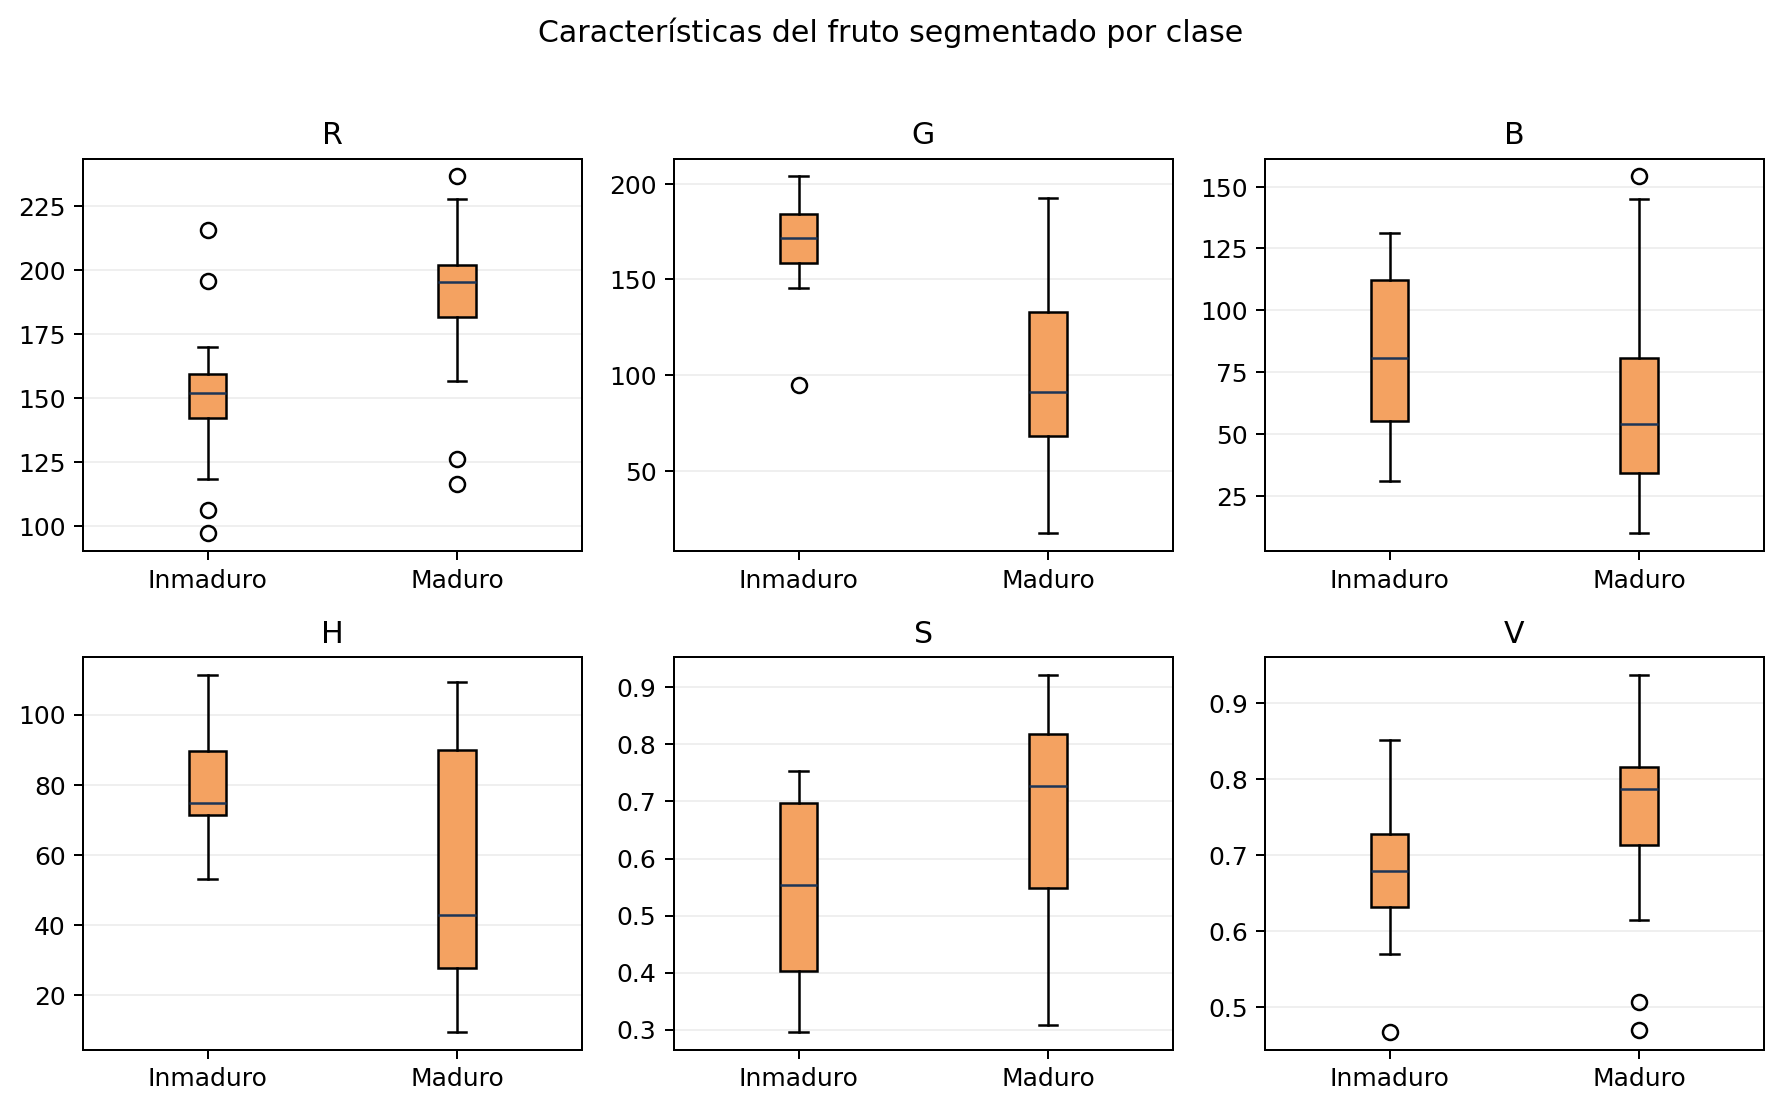
\includegraphics[width=0.88\textwidth]{feature_distributions.png}
\caption{Distribución de las seis características calculadas sobre la máscara
estimada. La separación de las clases es especialmente clara en R, G y H.}
\end{figure}

Los tomates maduros presentan un canal R alto y canales G/B bajos, mientras que los
inmaduros presentan un canal G alto. El tono H también cambia: el promedio del fruto
maduro es cercano a $48^\circ$, frente a $78^\circ$ en el inmaduro. Saturación y
valor aportan información, pero son más sensibles a iluminación, reflejos y fondo.
Por ello, la selección basada en análisis usa $[R,G,H]$: son variables con una
diferencia de clase grande y una interpretación directa, evitando añadir variables
redundantes sin evidencia adicional.

\section{Segmentación mediante K-Means}

\subsection{Configuración}

Para cada imagen y cada combinación se ajusta un K-Means independiente con:

\begin{itemize}[leftmargin=1.5em]
    \item $k=2$ clusters: fruto y fondo;
    \item inicialización \texttt{k-means++}, 10 reinicios;
    \item máximo de 300 iteraciones y tolerancia $10^{-4}$;
    \item semilla $20260913$;
    \item muestra uniforme de hasta 12\,000 píxeles para ajustar K-Means y
    predicción sobre todos los píxeles redimensionados.
\end{itemize}

La etiqueta interna del cluster no tiene significado, por lo que no se usa el
orden de los centroides. Para seleccionar el cluster del fruto sin consultar la
anotación, se calcula un puntaje de objeto que combina coherencia del componente
conectado mayor, centralidad, saturación, valor HSV, un prior suave de área y una
penalización por tocar el borde. La máscara de referencia se usa después solamente
para calcular Jaccard:

\begin{equation}
J(A,B)=\frac{|A\cap B|}{|A\cup B|}.
\end{equation}

\subsection{Comparación de canales}

La elección de la combinación se realiza con el promedio del conjunto de desarrollo
(entrenamiento más validación). El test se muestra solo como evaluación final.

\begin{table}[H]
\centering
\scriptsize
\caption{Jaccard medio y desviación estándar. La selección se basa en desarrollo.}
\begin{tabular}{lrrrr}
\toprule
Combinación & Desarrollo: media & Desarrollo: DE & Test: media & Test: DE \\
\midrule
R   & 0.533 & 0.221 & 0.442 & 0.300 \\
G   & 0.512 & 0.247 & 0.409 & 0.302 \\
B   & 0.511 & 0.296 & 0.490 & 0.335 \\
RG  & 0.553 & 0.232 & 0.483 & 0.328 \\
RB  & \textbf{0.560} & 0.254 & 0.465 & 0.361 \\
GB  & 0.515 & 0.287 & 0.457 & 0.351 \\
RGB & 0.547 & 0.257 & 0.455 & 0.348 \\
\bottomrule
\end{tabular}
\end{table}

\begin{figure}[H]
\centering
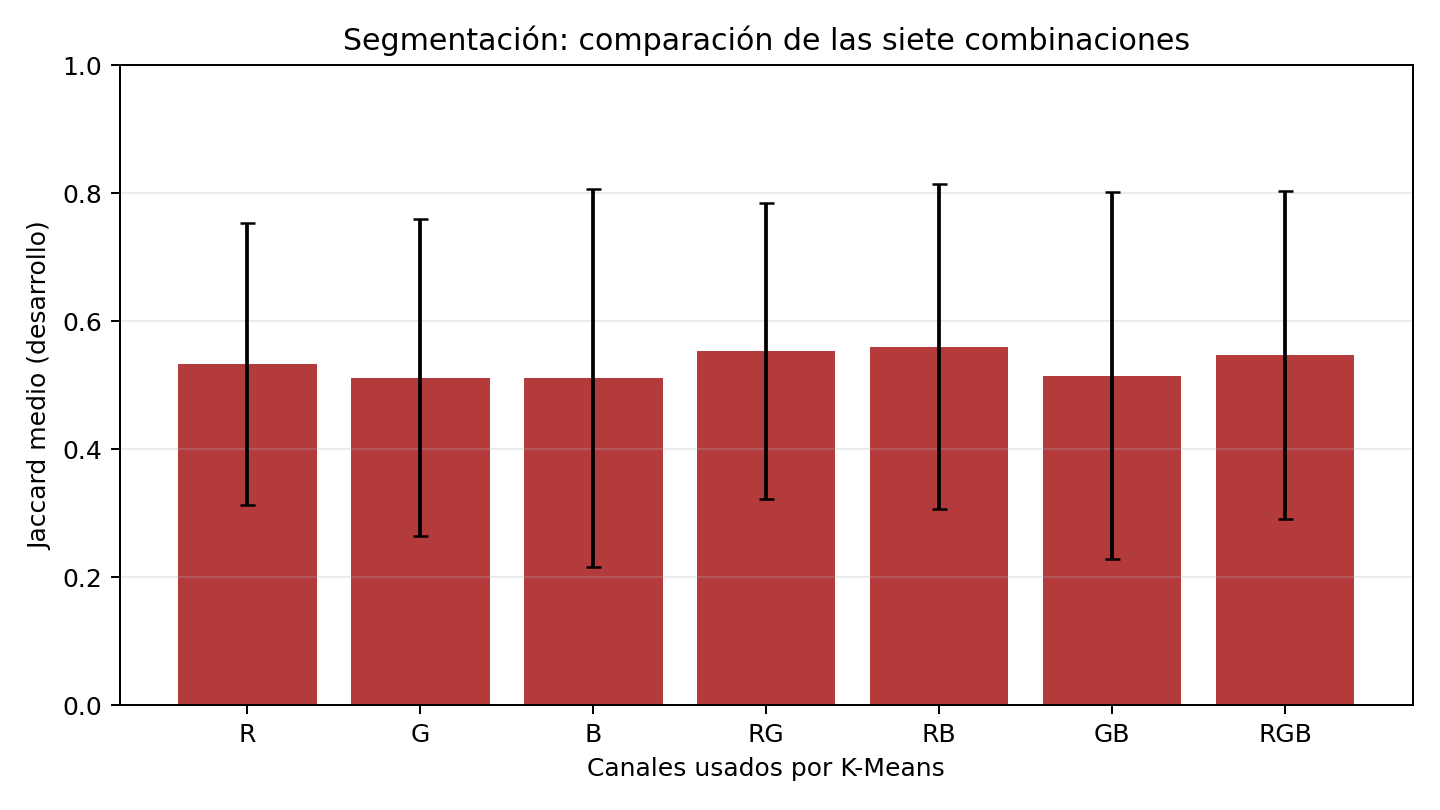
\includegraphics[width=0.86\textwidth]{segmentation_jaccard.png}
\caption{Comparación de Jaccard en desarrollo para las siete combinaciones. Las
barras de error son desviaciones estándar entre imágenes.}
\end{figure}

RB se selecciona porque alcanza el mejor promedio de desarrollo ($0.560$). La
ventaja sobre RG ($0.553$) y RGB ($0.547$) es pequeña, por lo que no se debe
interpretar como una superioridad universal: el test baja a $0.465$ y mantiene una
variabilidad alta. En este conjunto, B ayuda a distinguir tomates brillantes u
oscuros en escenas donde R y G por sí solos se confunden con el fondo, pero K-Means
con solo dos clusters no separa siempre fondos complejos, hojas, platos o madera.

\begin{figure}[H]
\centering
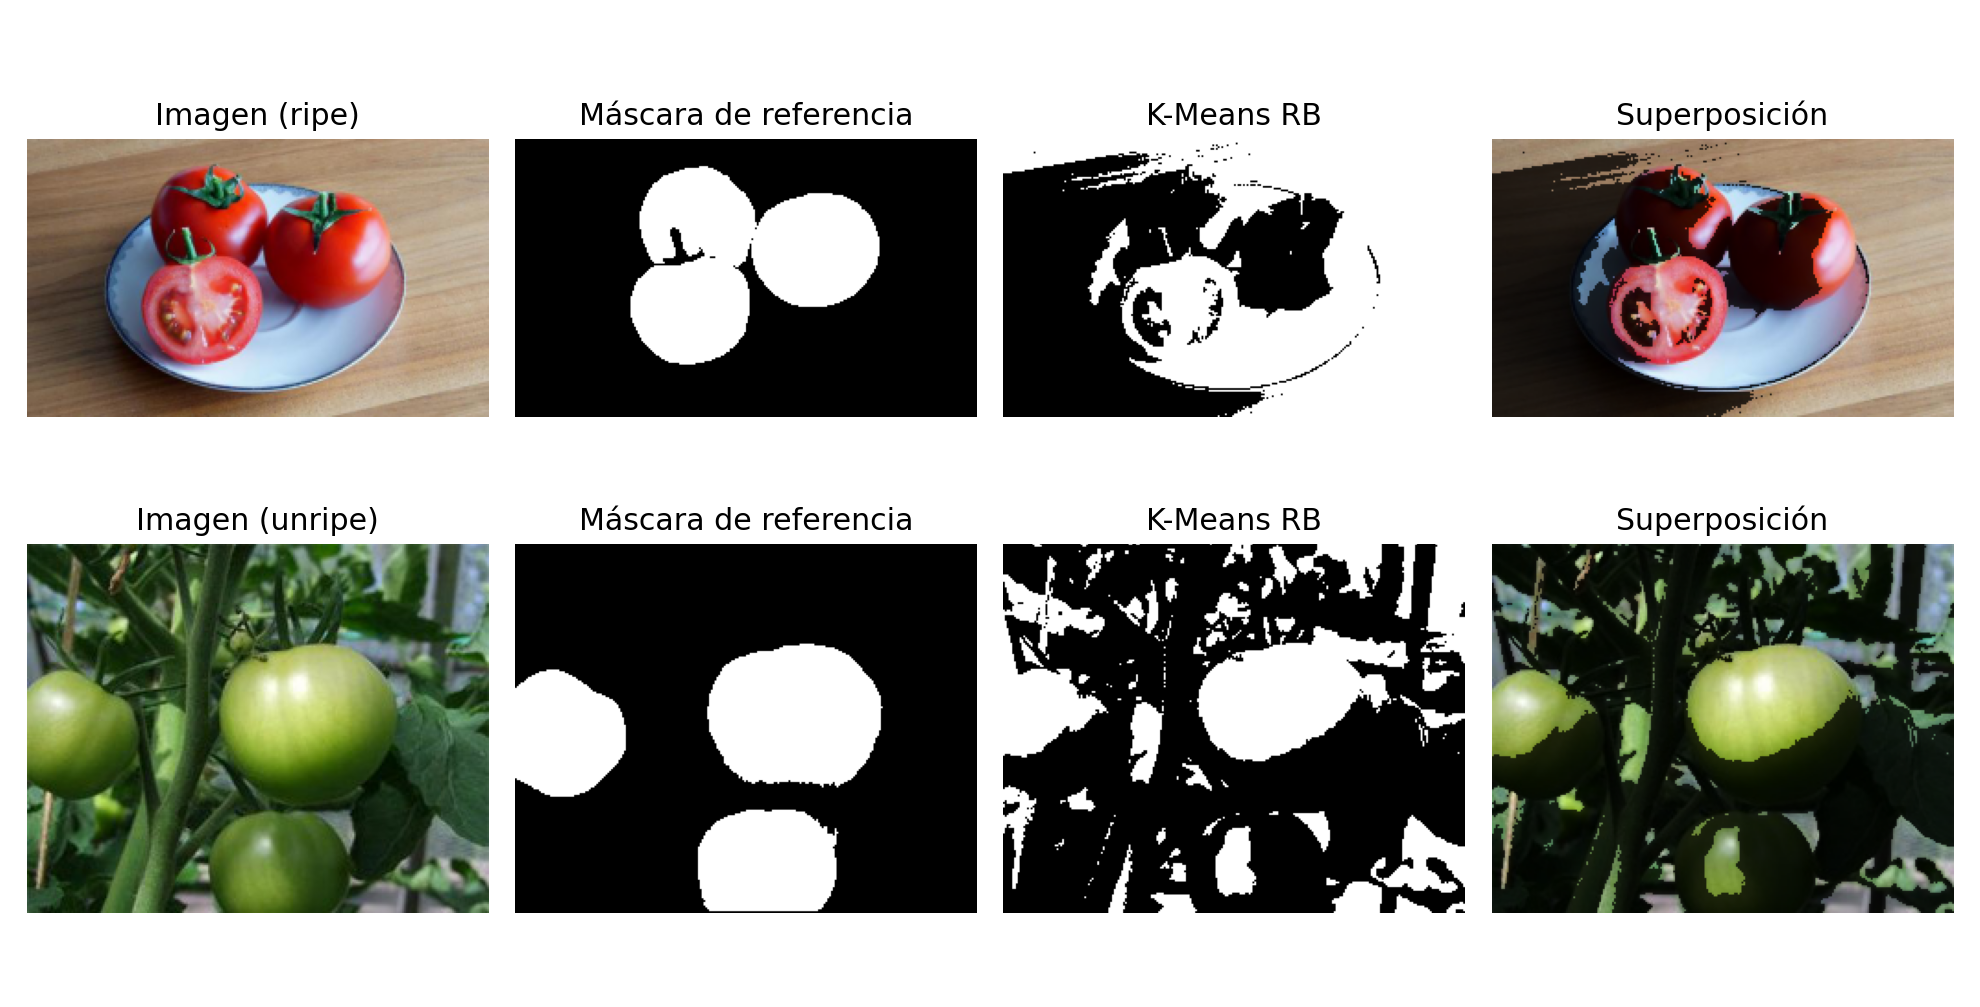
\includegraphics[width=0.98\textwidth]{segmentation_examples.png}
\caption{Ejemplos representativos para RB: imagen, máscara de referencia, máscara
estimada y superposición. Las imperfecciones muestran la limitación de usar color
global con solo dos clusters.}
\end{figure}

\section{Extracción y selección de características}

Con la máscara RB seleccionada, cada imagen queda representada por el promedio de
los píxeles del fruto estimado:

\begin{equation}
\mathbf{x}=[\bar R,\bar G,\bar B,\bar H,\bar S,\bar V].
\end{equation}

RGB se conserva en la escala 0--255; H se expresa en grados y S/V en $[0,1]$.
Antes de cada clasificador se aplica estandarización $z=(x-\mu)/\sigma$ ajustada
solo con entrenamiento. La segmentación estimada se usa tanto en entrenamiento como
en validación y test, por lo que la clasificación mide el sistema completo y no una
versión artificial con máscaras perfectas.

\subsection{Selección basada en análisis}

Se selecciona $[R,G,H]$. R captura la dominante roja del maduro, G la dominante
verde del inmaduro y H resume la posición de color de manera complementaria. Esta
decisión se fundamenta en los promedios de la Tabla 3 y en las distribuciones de la
Figura 2.

\subsection{Selección secuencial hacia adelante}

Como segunda estrategia se implementa SFS con validación cruzada estratificada de
cinco particiones sobre entrenamiento. En cada paso se añade la variable que
maximiza el AUC medio de un pipeline estandarización + GaussianNB. Para reducir la
inestabilidad de una muestra pequeña, se permite continuar mientras el AUC no caiga
más de 0.01; se detiene a lo más en cuatro variables. El orden obtenido fue:

\begin{table}[H]
\centering
\caption{Traza de SFS sobre entrenamiento.}
\begin{tabular}{crr}
\toprule
Paso & Variable añadida & AUC medio CV \\
\midrule
1 & G & 0.988 \\
2 & R & 0.983 \\
3 & B & 0.983 \\
4 & S & 0.983 \\
\bottomrule
\end{tabular}
\end{table}

El subconjunto final es $[G,R,B,S]$. Coincide parcialmente con la selección por
análisis: ambas conservan R y G. SFS incorpora B y S, posiblemente porque capturan
variaciones de iluminación, reflejos y saturación que no aparecen con la misma
claridad en la inspección de medias.

\section{Clasificación bayesiana y regla de decisión}

Para cada subconjunto se ajusta GaussianNB. Para la clase positiva maduro, el
clasificador produce $s(\mathbf{x})=P(y=1\mid\mathbf{x})$. La regla de decisión es

\begin{equation}
\hat y=\begin{cases}
1 & s(\mathbf{x})\geq \tau,\\
0 & s(\mathbf{x})<\tau.
\end{cases}
\end{equation}

Esto es equivalente a una razón de verosimilitudes con un umbral que incorpora las
probabilidades a priori y los costos de error. El umbral $\tau$ se fija con el
índice de Youden sobre validación:

\begin{equation}
J_{Y}(\tau)=\operatorname{sensibilidad}(\tau)-\operatorname{FPR}(\tau),
\qquad \tau^*=\arg\max_{\tau}J_Y(\tau).
\end{equation}

Youden se elige porque busca simultáneamente sensibilidad y especificidad, sin
asumir un costo clínico o comercial específico para cada tipo de error. Luego el
modelo se reentrena con entrenamiento más validación, conservando $\tau^*$, y se
evalúa sobre test.

\begin{table}[H]
\centering
\scriptsize
\caption{Evaluación con el umbral seleccionado por Youden.}
\begin{tabular}{llrrrrrr}
\toprule
Modelo & Conjunto & $\tau^*$ & AUC & Exactitud & Sens. & Espec. & F1 \\
\midrule
Bayes + análisis & Validación & 0.984 & 0.976 & 0.923 & 0.857 & 1.000 & 0.923 \\
Bayes + SFS      & Validación & 0.357 & 0.952 & 0.923 & 1.000 & 0.833 & 0.875 \\
PCA + Bayes      & Validación & 0.827 & 0.952 & 0.923 & 0.857 & 1.000 & 0.923 \\
\midrule
Bayes + análisis & Test & 0.984 & 0.833 & 0.846 & 0.833 & 0.857 & 0.833 \\
Bayes + SFS      & Test & 0.357 & \textbf{0.929} & 0.846 & 0.833 & 0.857 & 0.833 \\
PCA + Bayes      & Test & 0.827 & 0.857 & 0.846 & 0.833 & 0.857 & 0.833 \\
\bottomrule
\end{tabular}
\end{table}

En test, SFS obtiene el mayor AUC y por tanto ordena mejor los casos según su
probabilidad, pero la exactitud es idéntica para las tres alternativas: 11 de 13
imágenes. El conjunto de test es pequeño, por lo que una sola imagen cambia la
exactitud en aproximadamente 7.7 puntos porcentuales.

\begin{figure}[H]
\centering
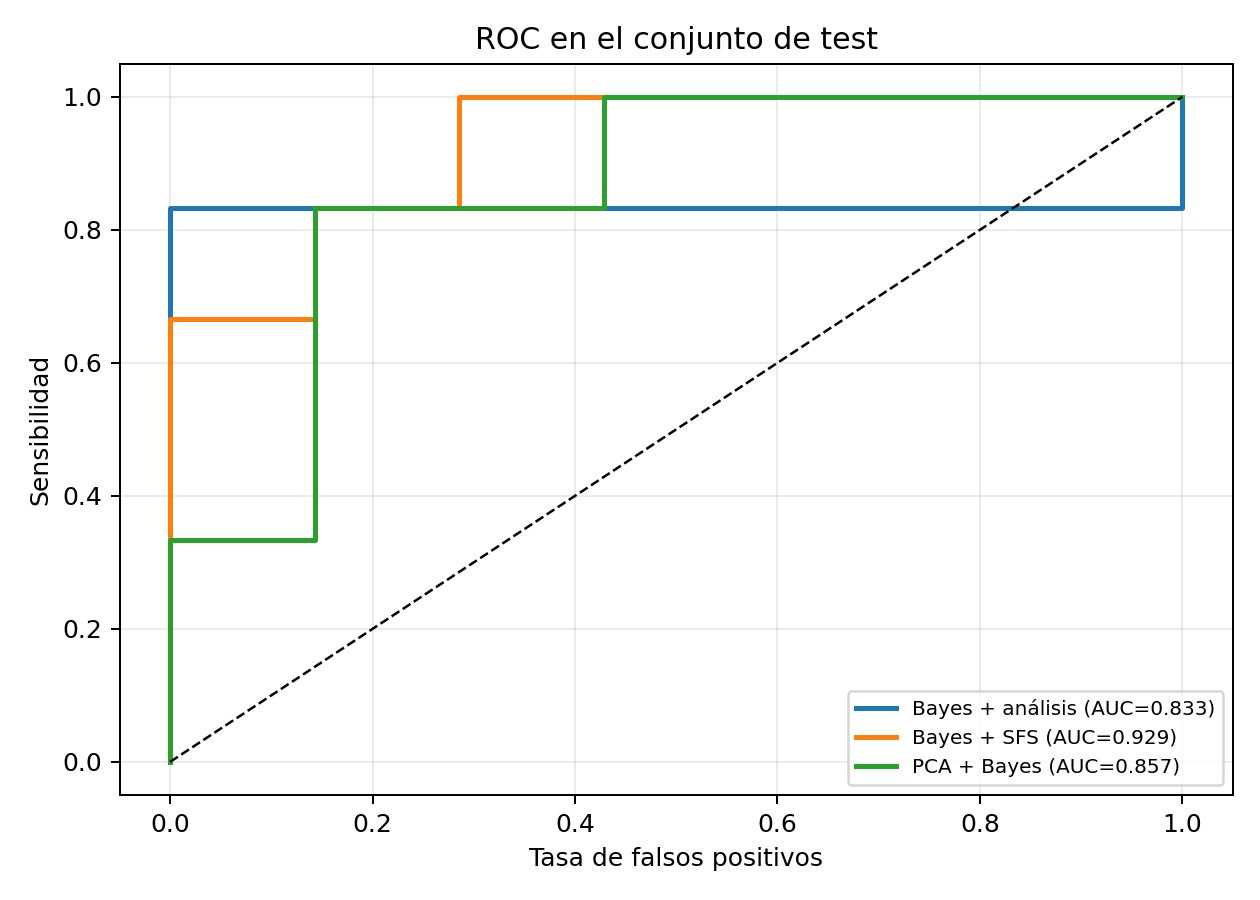
\includegraphics[width=0.78\textwidth]{roc_test.png}
\caption{Curvas ROC y AUC en test. El umbral operativo no se optimiza usando esta
figura; fue fijado previamente en validación.}
\end{figure}

\section{PCA + Bayes}

PCA se ajusta sobre las seis variables estandarizadas usando únicamente
entrenamiento. La cantidad de componentes se fija como el menor número que alcanza
95\% de varianza acumulada. Los valores obtenidos son:

\begin{table}[H]
\centering
\scriptsize
\caption{PCA ajustado sobre entrenamiento.}
\begin{tabular}{crrr}
\toprule
Componente & Autovalor & Varianza individual & Acumulada \\
\midrule
PC1 & 3.532 & 57.225\% & 57.225\% \\
PC2 & 1.892 & 30.663\% & 87.888\% \\
PC3 & 0.449 & 7.271\%  & 95.158\% \\
PC4 & 0.249 & 4.040\%  & 99.198\% \\
PC5 & 0.039 & 0.635\%  & 99.833\% \\
PC6 & 0.010 & 0.167\%  & 100.000\% \\
\bottomrule
\end{tabular}
\end{table}

Se usan tres componentes porque son suficientes para superar el 95\% sin conservar
las seis coordenadas originales. El clasificador GaussianNB se entrena sobre
$[PC1,PC2,PC3]$ y se evalúa con el mismo umbral de Youden que las alternativas
anteriores. En este experimento PCA no mejora la exactitud frente a la selección de
variables, y su AUC de test ($0.857$) queda por debajo de SFS ($0.929$).

\begin{figure}[H]
\centering
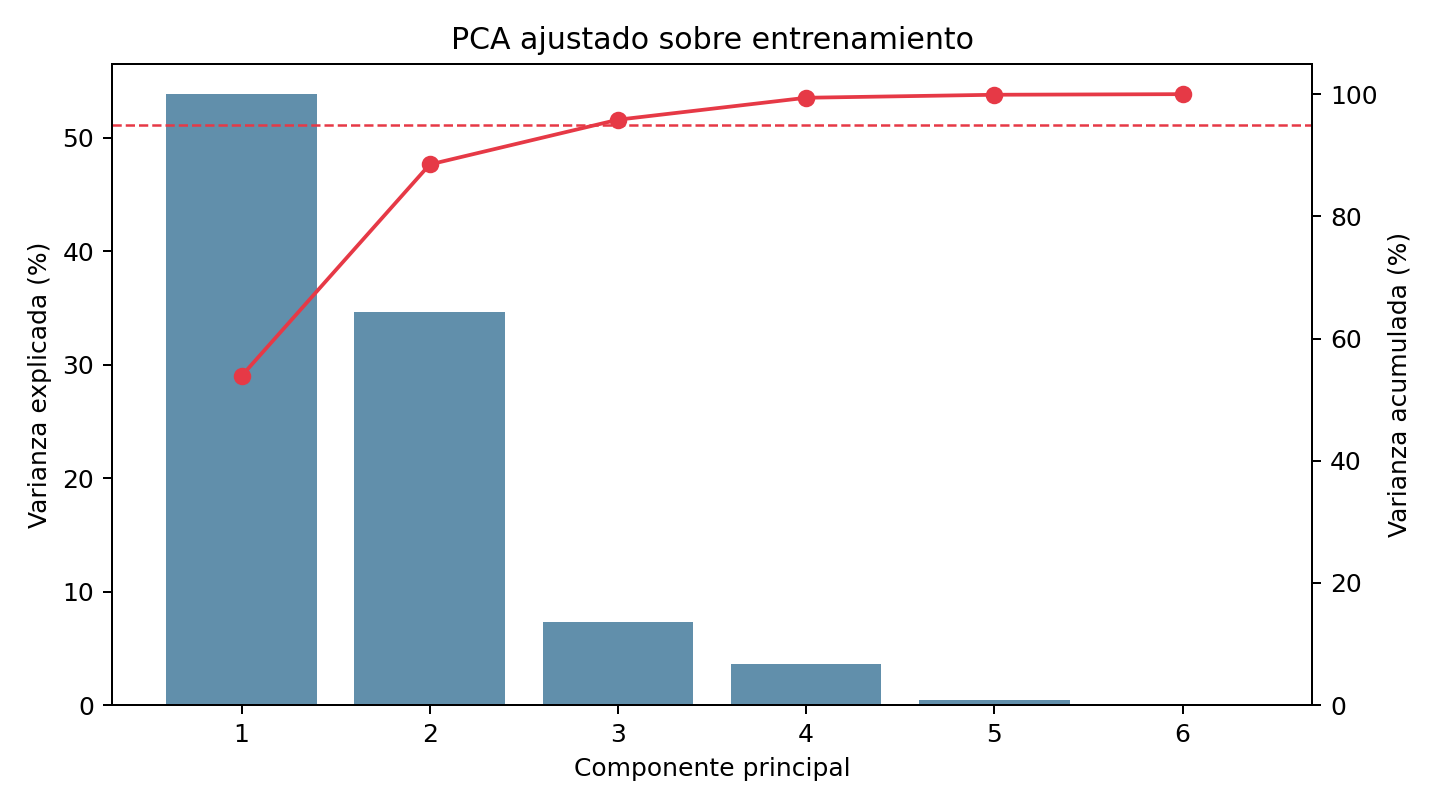
\includegraphics[width=0.84\textwidth]{pca_variance.png}
\caption{Varianza individual y acumulada. La línea horizontal marca el 95\% usado
para elegir tres componentes.}
\end{figure}

\section{Relación entre segmentación y clasificación}

La calidad de la máscara es una fuente directa de error en las características: si
la máscara incluye hojas, plato o madera, los promedios RGB/HSV dejan de representar
solo al fruto. Para cuantificarlo se usa el clasificador de mejor AUC, Bayes + SFS,
y se compara Jaccard RB por imagen en el test.

\begin{table}[H]
\centering
\caption{Análisis integrado en test.}
\begin{tabular}{lr}
\toprule
Cantidad & Valor \\
\midrule
Jaccard RB medio en desarrollo & 0.560 \\
Jaccard RB medio en test & 0.465 \\
Jaccard medio cuando la clasificación es correcta & 0.538 \\
Jaccard medio cuando la clasificación falla & 0.068 \\
Correlación de Spearman entre Jaccard y acierto & 0.627 \\
Valor p exploratorio & 0.0219 \\
\bottomrule
\end{tabular}
\end{table}

Los errores de clasificación se concentran en imágenes con máscaras muy deficientes,
lo que respalda que la segmentación afecta el desempeño posterior. La correlación
debe interpretarse con cautela: solo hay 13 imágenes de test y la variable de acierto
es binaria. El resultado no prueba causalidad, pero sí identifica una limitación
operativa clara del sistema.

\section{Respuestas a las preguntas centrales}

\begin{enumerate}[leftmargin=1.7em]
    \item \textbf{Mejor combinación RGB:} RB, seleccionada por el mayor Jaccard medio
    de desarrollo ($0.560$).
    \item \textbf{Razón:} R y B combinan contraste cromático y de luminancia útil
    frente a fondos que se confunden con un solo canal; la diferencia es pequeña y
    depende de la escena.
    \item \textbf{Características discriminantes:} R alto en maduros, G alto en
    inmaduros y H desplazado entre ambas clases; S también es útil según SFS.
    \item \textbf{SFS:} $[G,R,B,S]$. Coincide con la selección exploratoria en R/G,
    pero añade B/S para absorber variación de iluminación y saturación.
    \item \textbf{Mejor clasificador:} Bayes + SFS por AUC de test ($0.929$); la
    exactitud de test queda empatada en $0.846$.
    \item \textbf{Punto de operación:} índice de Youden, elegido para equilibrar
    sensibilidad y especificidad sin costos de error especificados.
    \item \textbf{Número de componentes:} tres, porque la varianza acumulada alcanza
    $95.158\%$ en PC3.
    \item \textbf{¿PCA mejora?:} no en exactitud; obtiene $0.846$, igual que las
    selecciones, y AUC menor que SFS.
    \item \textbf{Efecto de segmentación:} las imágenes correctas tienen Jaccard
    medio $0.538$ y las incorrectas $0.068$; la contaminación del fruto deteriora
    las características y la decisión posterior.
\end{enumerate}

\section{Conclusiones y limitaciones}

Se implementó el flujo solicitado de extremo a extremo y se respetó la separación
por imagen y el aislamiento del test. La evidencia favorece RB para segmentación y
SFS para clasificación cuando se prioriza AUC. La inspección visual y los
estadísticos explican la utilidad de R, G y H, mientras que SFS detecta que B y S
aportan información complementaria. PCA logra una representación compacta, pero no
mejora el clasificador en esta partición.

Las conclusiones deben considerarse exploratorias. El conjunto tiene solo 62
imágenes, resoluciones y contextos muy variados, y el test contiene 13 imágenes.
Además, K-Means con dos clusters y características RGB globales no modela
explícitamente textura, bordes ni múltiples objetos. Un siguiente desarrollo podría
incorporar postprocesamiento morfológico, más clusters, características espaciales,
validación cruzada repetida o una segmentación supervisada, manteniendo la misma
separación estricta del test.

\section*{Reproducibilidad}

El código ejecutable está en \texttt{tomato\_project.py}. Desde el directorio del
proyecto se puede regenerar el conjunto de resultados con:

\begin{verbatim}
python -X utf8 tomato_project.py
pdflatex -interaction=nonstopmode -halt-on-error report.tex
pdflatex -interaction=nonstopmode -halt-on-error report.tex
\end{verbatim}

El primer comando genera las tablas CSV, el resumen JSON y las figuras en
\texttt{results/}. Los comandos LaTeX generan este informe a partir de esos
artefactos.

\end{document}
